\documentclass[12pt]{article}	

\usepackage[margin=1in]{geometry}
\usepackage{amsmath,amssymb,amsthm}
\usepackage{caption}
\usepackage{subcaption}
\usepackage{graphicx}
\usepackage{url}
\usepackage{mathrsfs}
\newtheorem{theorem}{Theorem}
\newtheorem{notation}{Notation}
\newtheorem{claim}{Claim}
\newtheorem{lemma}{Lemma}
\newtheorem{definition}{Definition}
\renewcommand{\qedsymbol}{$\blacksquare$}
\newtheorem*{remark}{Remark}
\usepackage[utf8]{inputenc}

\usepackage{listings}
\usepackage{xcolor}

\definecolor{codegreen}{rgb}{0,0.6,0}
\definecolor{codegray}{rgb}{0.5,0.5,0.5}
\definecolor{codepurple}{rgb}{0.58,0,0.82}
\definecolor{backcolour}{rgb}{1,1,1}
\definecolor{grey}{rgb}{0.70, 0.70, 0.70}

\lstdefinestyle{mystyle}{
	backgroundcolor=\color{backcolour},   
	commentstyle=\color{grey},
	keywordstyle=\color{codepurple},
	numberstyle=\tiny\color{codegray},
	stringstyle=\color{codegreen},
	basicstyle=\ttfamily\footnotesize,
	breakatwhitespace=false,         
	breaklines=true,                 
	captionpos=b,                    
	keepspaces=true,                 
	numbers=left,                    
	numbersep=5pt,                  
	showspaces=false,                
	showstringspaces=false,
	showtabs=false,                  
	tabsize=2
}

\lstset{style=mystyle}


\begin{document}
	Arun Suresh
	\begin{center}
		Computational Physics 1 - Homework 9
	\end{center} 
	{\rule{\linewidth}{0.1mm} }

For my assignment, I chose to run the hturb example that was provided in the turb example library for the class. This example is concerned with simulating turbulence in a box. The simulation was run twice using two different Riemann solvers. The Riemann solvers used were the ones suggested in the homework assignment. For the first run, the simulation used the ROE solver, which uses the linearized version of the jacobian, which is then solved exactly at the point of discontinuity. The second run made use of the HLLC solver which makes uses of Godunov-type fluxes and related integral equations to solve. \\\\
The simulation consisted of a box fragmented into 64 smaller boxes where problem was solved - the riemann solver was then used to glue together these smaller fragments to reconstruct the entire box. The athinput.turb file was edited to have tlim = 0.7. This means that the solution was solved for 8 time steps (0s to 0.7s with dt=0.1). This was done because, each smaller fragment produced 8 files, and so for a single time step, there were 64$\times$8 = 512 ouput files, and if I wanted the simulation to last for 10 seconds there would be 51200 files. Setting aside issue about filling up space, I also noticed that the $join\_all\_vtk.sh$ and $join\_vtk++.c$ visualization scripts (that produces a single metadata file for VisIt) that was included with Athena did not seem to run because of a few permission issues - and so, 51200 files would be a little too much for me to parse manually. So tlim was set to a relatively low value. \\\\
The output obtained was then trasferred to my local computer where I once again tried to use the join scripts and failed because of permission issues in my computer (Because of some Xcode issues in my local computer). So I ended up manually visualizing the smaller fragments using VisIt by creating a correlation plot where I overlayed different fragments to visualize them side by side. Since it was a tedious job to merge all 63$\times$8 files on visnek manually ($\times$ 2 for the two solvers), I selected the first 12 fragments (which made up the bottom left 1/5th of the box)	for this assignment as a proof of concept. I would like to follow this up with an additional assignment submission with the full result after I figure out how to use the $c$ scripts included in the visualization folder.\\\\

For the visualization, the total energy of the fluid across the box and its time evolution were plotted. This choice was made because analyzing turbulence would yield meaningful results through observing the energy profile. All that being said, presented below are the results that were observed. \newpage \noindent \textbf{Total Energy:}\\
\begin{figure}[h]
	\centering
	\begin{subfigure}[h]{0.4500\textwidth}
		\centering
		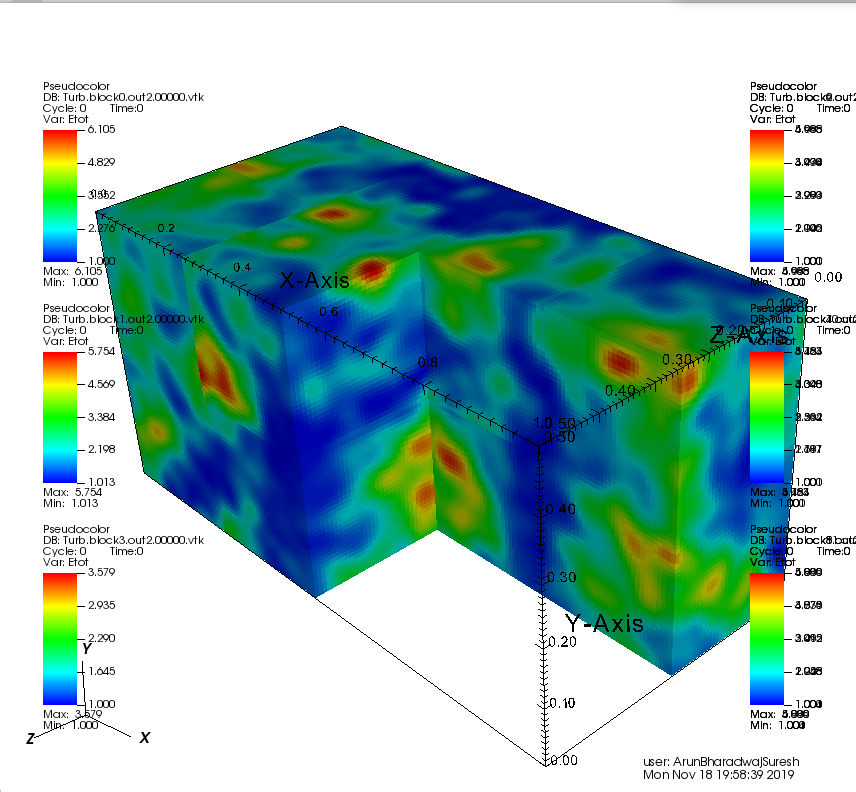
\includegraphics[width=\textwidth]{roet0.png}
		\caption{Roe: t =0}
	\end{subfigure}
	\begin{subfigure}[h]{0.4500\textwidth}
		\centering
		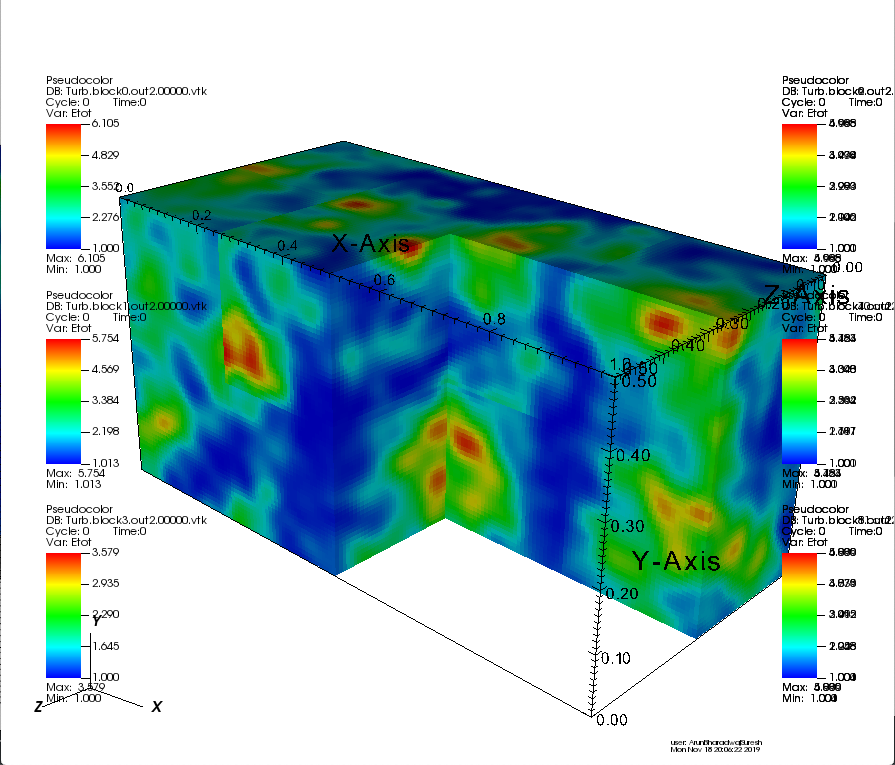
\includegraphics[width=\textwidth]{hllct0.png}
		\caption{Hllc: t = 0}
	\end{subfigure}
\end{figure}\\\\
\begin{figure}[h]
	\centering
	\begin{subfigure}[h]{0.4500\textwidth}
		\centering
		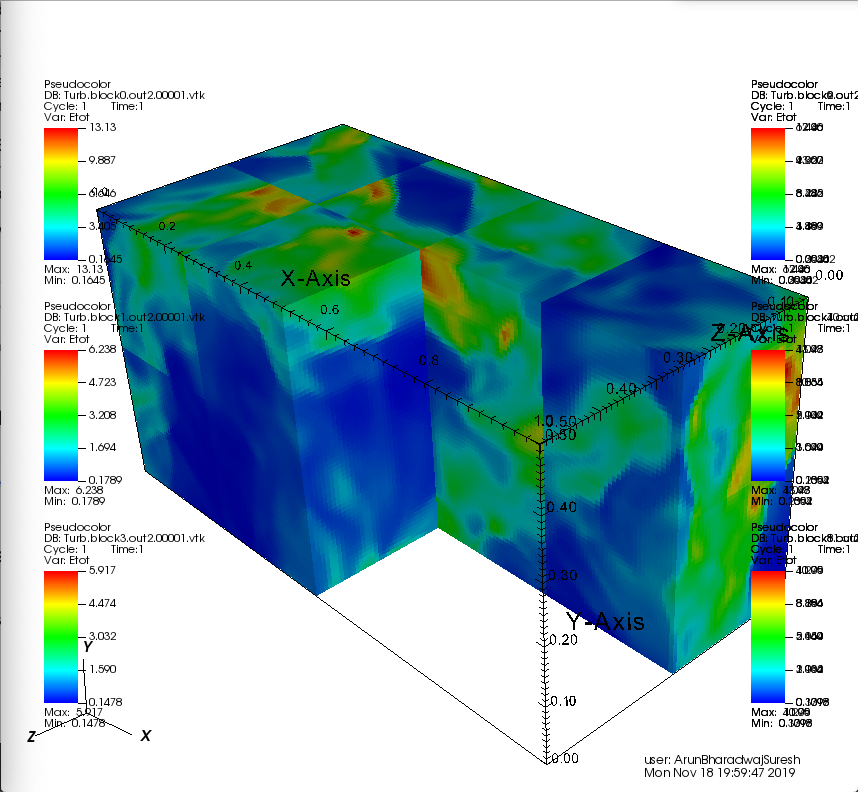
\includegraphics[width=\textwidth]{roet1.png}
		\caption{Roe: t = 0.1}
	\end{subfigure}
	\begin{subfigure}[h]{0.4500\textwidth}
		\centering
		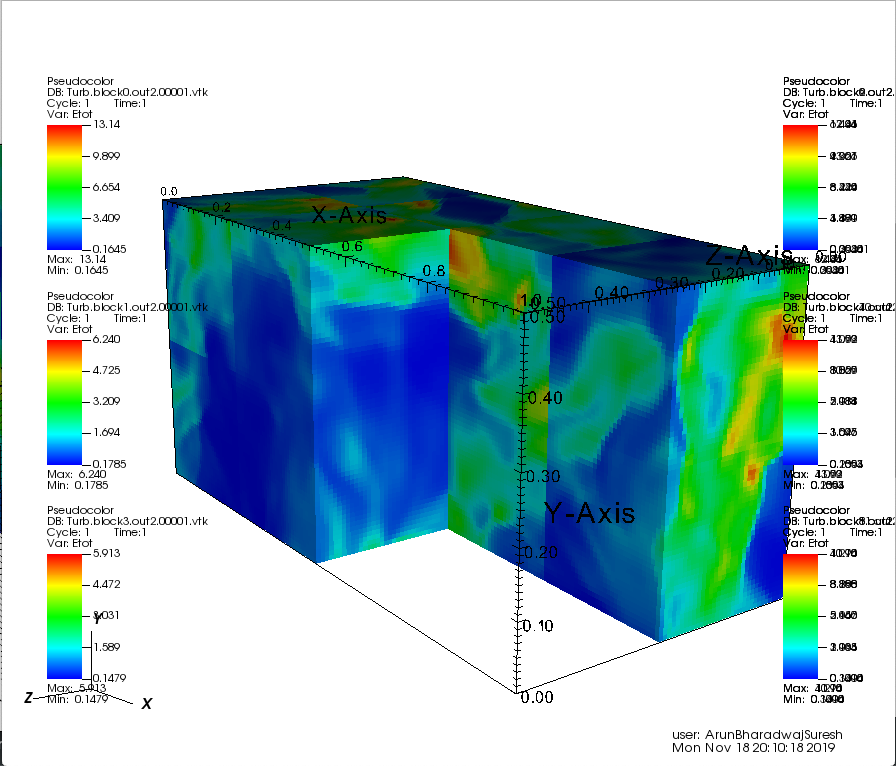
\includegraphics[width=\textwidth]{hllct1.png}
		\caption{Hllc: t = 0.1}
	\end{subfigure}
\end{figure}\\\\
\begin{figure}[h]
	\centering
	\begin{subfigure}[h]{0.4500\textwidth}
		\centering
		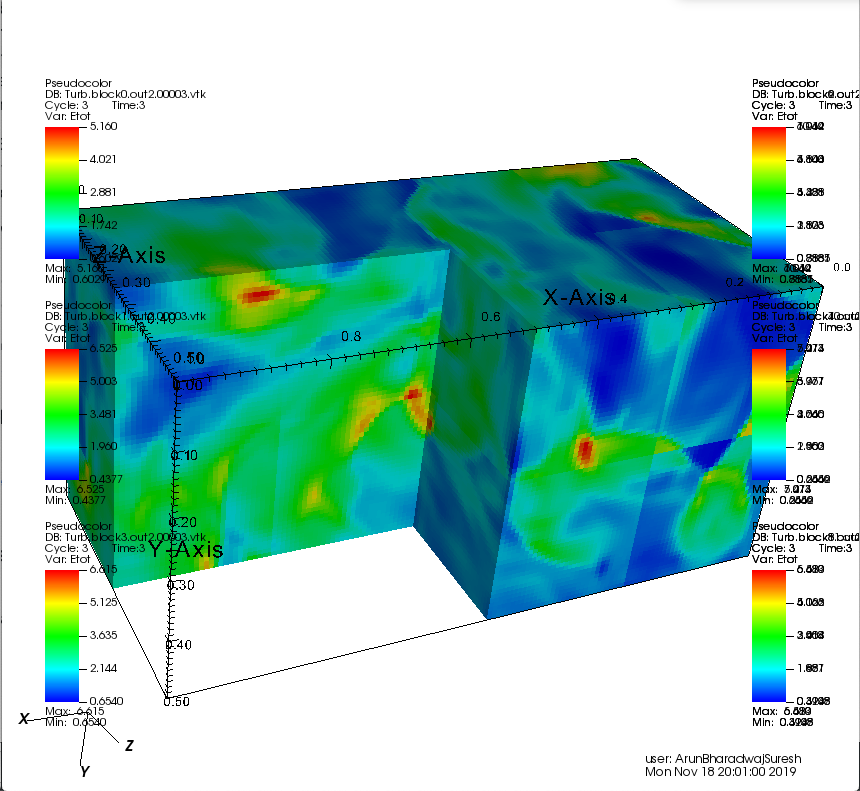
\includegraphics[width=\textwidth]{roet3.png}
		\caption{Roe: t = 0.3}
	\end{subfigure}
	\begin{subfigure}[h]{0.4500\textwidth}
		\centering
		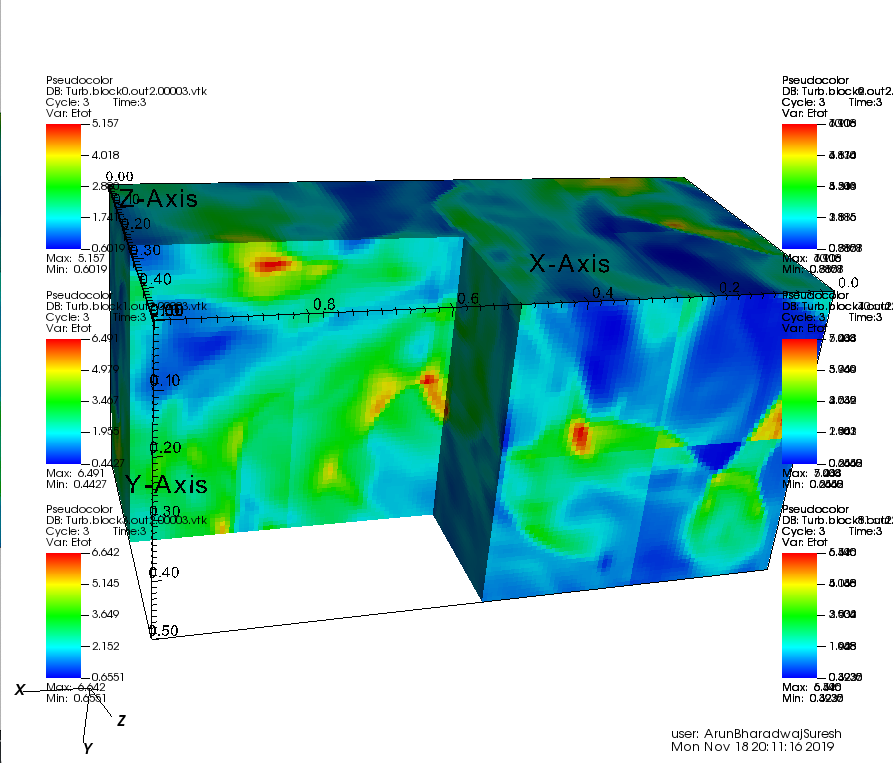
\includegraphics[width=\textwidth]{hllct3.png}
		\caption{Hllc: t = 0.3}
	\end{subfigure}
\end{figure}\\\\
\begin{figure}[h]
	\centering
	\begin{subfigure}[h]{0.4500\textwidth}
		\centering
		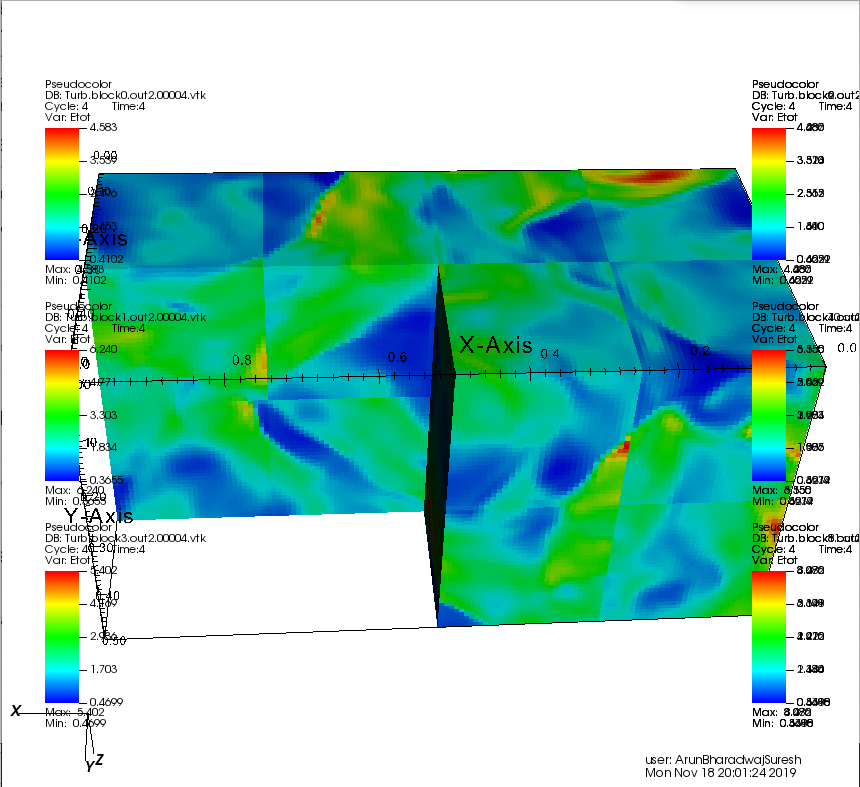
\includegraphics[width=\textwidth]{roet4.png}
		\caption{Roe: t = 0.4}
	\end{subfigure}
	\begin{subfigure}[h]{0.4500\textwidth}
		\centering
		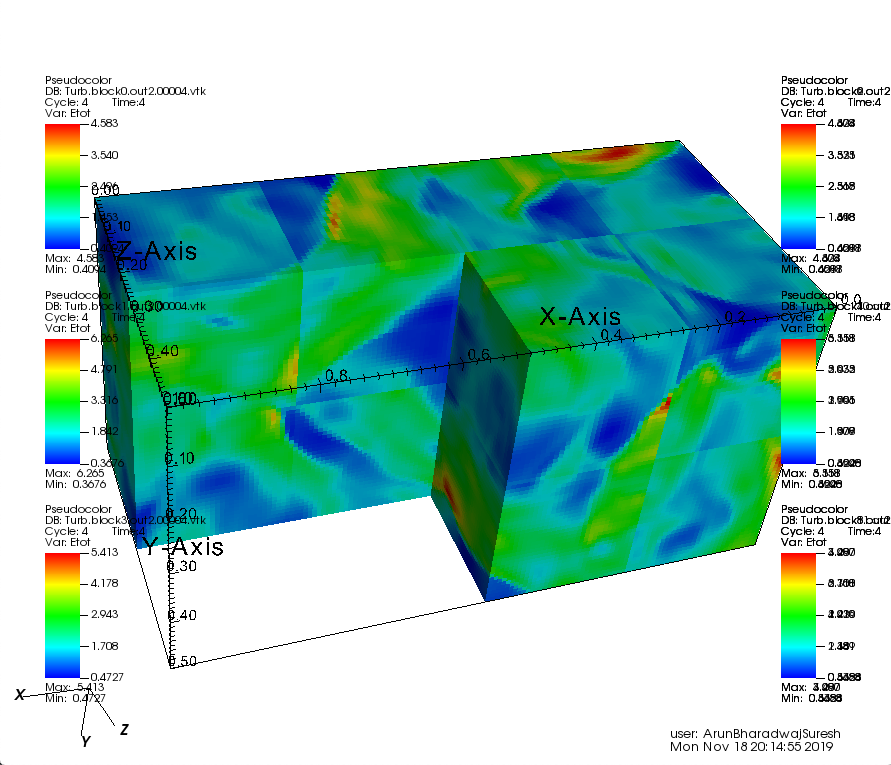
\includegraphics[width=\textwidth]{hllct4.png}
		\caption{Hllc: t = 0.4}
	\end{subfigure}
\end{figure}\\\\
\begin{figure}[h]
	\centering
	\begin{subfigure}[h]{0.4500\textwidth}
		\centering
		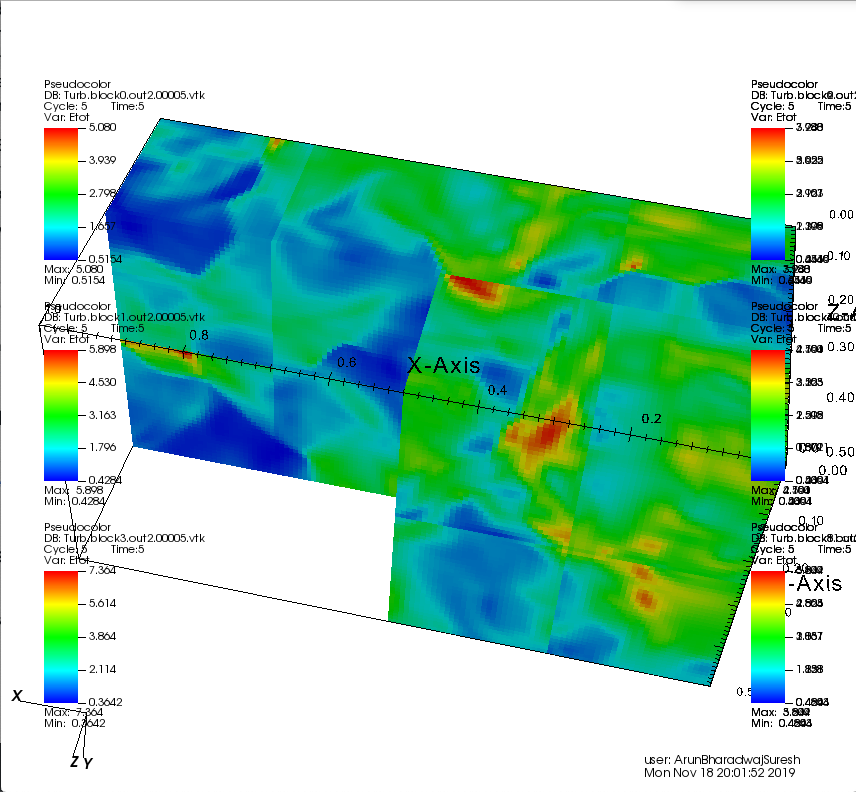
\includegraphics[width=\textwidth]{roet5.png}
		\caption{Roe: t = 0.5}
	\end{subfigure}
	\begin{subfigure}[h]{0.4500\textwidth}
		\centering
		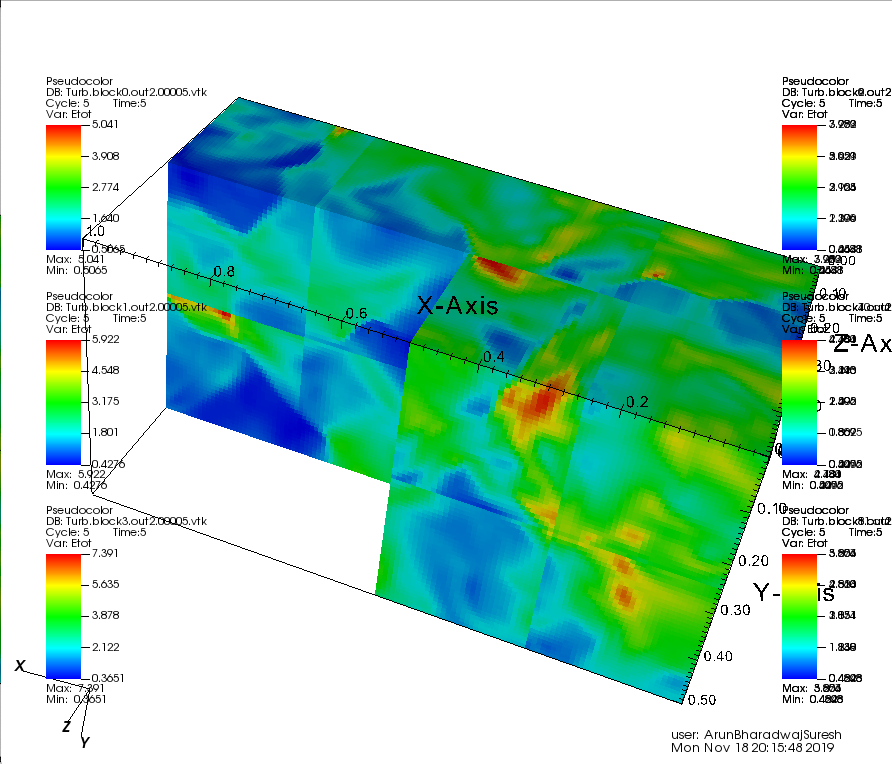
\includegraphics[width=\textwidth]{hllct5.png}
		\caption{Hllc: t = 0.5}
	\end{subfigure}
\end{figure}
\begin{figure}[h]
	\centering
	\begin{subfigure}[h]{0.4500\textwidth}
		\centering
		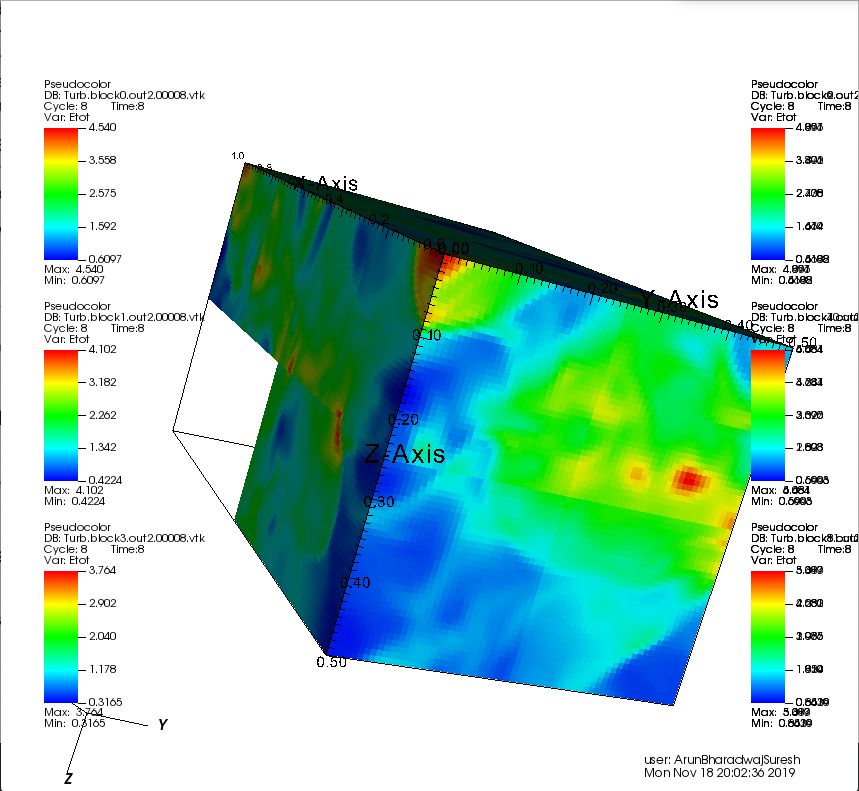
\includegraphics[width=\textwidth]{roet8a.png}
		\caption{Roe: t = 0.7 view: back}
	\end{subfigure}
	\begin{subfigure}[h]{0.4500\textwidth}
		\centering
		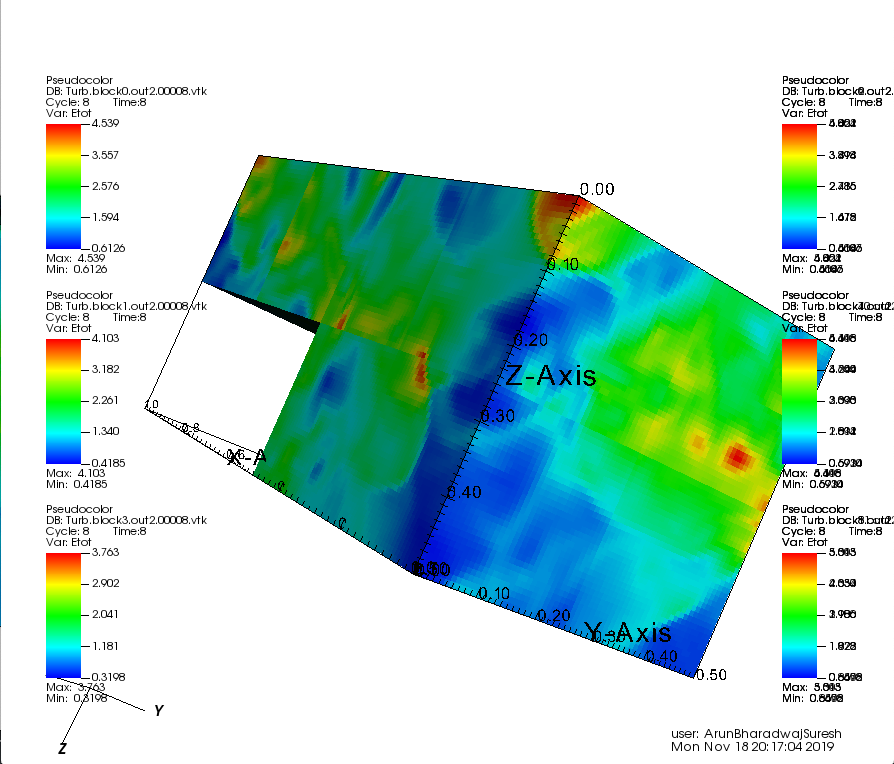
\includegraphics[width=\textwidth]{hllct8a.png}
		\caption{Hllc: t = 0.7 view: back}
	\end{subfigure}
\end{figure}
\begin{figure}[h]
\centering
\begin{subfigure}[h]{0.4500\textwidth}
	\centering
	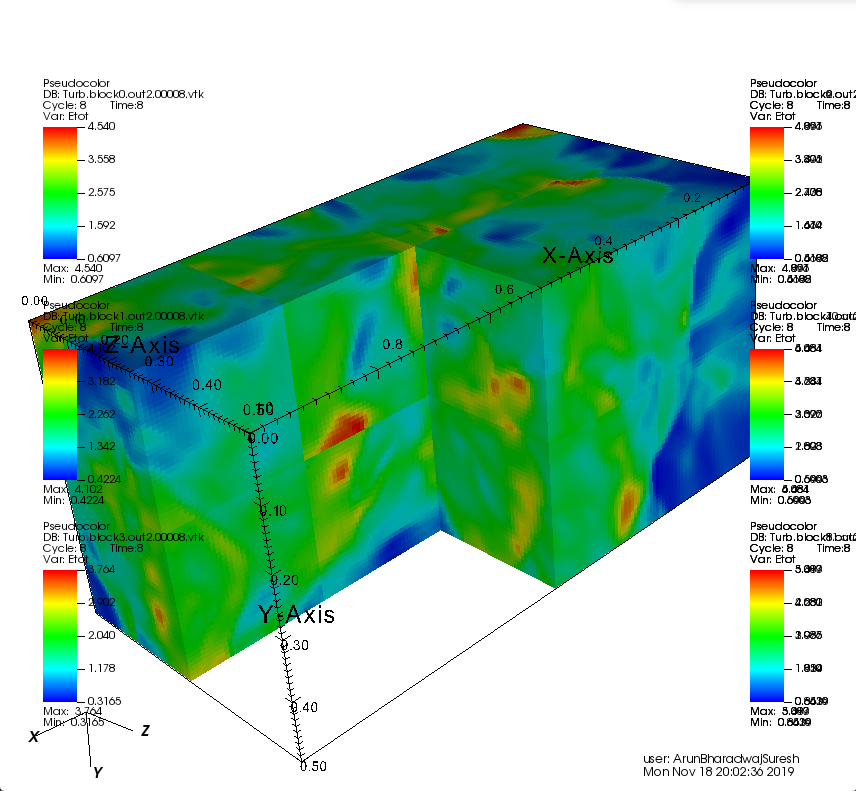
\includegraphics[width=\textwidth]{roet8b.png}
	\caption{Roe: t = 0.7 view: front}
\end{subfigure}
\begin{subfigure}[h]{0.4500\textwidth}
	\centering
	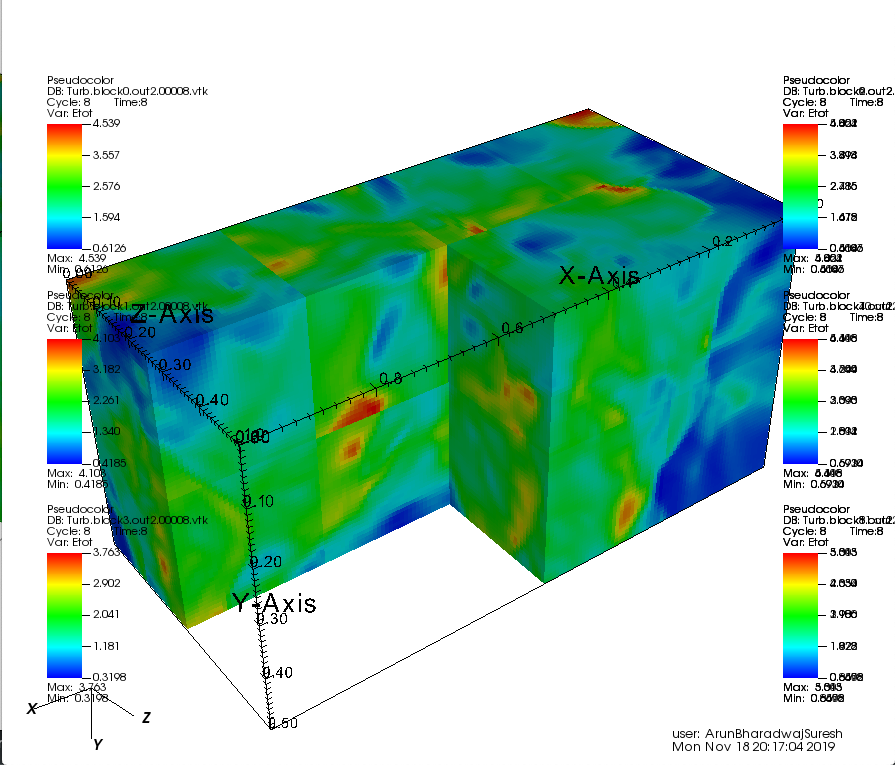
\includegraphics[width=\textwidth]{hllct8b.png}
	\caption{Hllc: t = 0.7 view: front}
\end{subfigure}
\end{figure}\\\\\\\\\\\\\\\\\\\\\\\\\\\\\\\\\\\\\\\\\\\\\\\\\\\\\\\\\\\\\\
It is apparent that both Roe and HLLC solvers very produce similar results. Upon very close inspection, we notice that the HLLC does a slightly better job at gluing the fragments than Roe. This can be seen a bit easily in the front view of the box, on the rear end and the lower side of the L cut, when t = 0.7 - where the lines that join the boxes are smoothed out much better than the Roe solver. But other than very specific details like that - both outputs seem to coincide very well. The only realistic way I was able to say that these results were from two different runs by eyeballing - were because of the different values at the color index during the different time frames.  \\\\
This close similarity between the two solvers, may also be be observed because the visualization did not make use of the entire box, but instead just a small part of it. Perhaps in areas with much more serious turbulence, the differences could be much more significant. I hope to answer this question in a follow up assignment submission where I analyze the entire box (after I figure out how to run the C script). 

\end{document}